\section{Introduction}
\label{sec:introduction}

\begin{figure}[h]
  \includegraphics[width=\linewidth]{media/caption2img}
  \caption[Caption to Image]{Images generated given a captioning text \cite{gan_t2i:2016}}
  \label{fig:caption2img}
\end{figure}
While sampling from generative models has by itself interesting applications, such as producing images given a caption as seen in Figure \ref{fig:caption2img}, there are many applications covering various different areas.
A subset of these applications include
image denoising, % TODO: citation
image impainting, % TODO: citation
text-to-speech, % TODO: citation, e.g. WaveNet
machine translation, % (neural?) TODO: e.g. NMT w/ VAE
and semi-supervised learning, for example discussed in \ref{ssub:cvae}.
\\\\

%Directed generative models are a wide class of models used for generating samples from an unknown distribution $p_\mathrm{data}$.
%The models presented in this article will approximate $p_\mathrm{data}$ with $p_\mathrm{model}$ which enables us to draw samples from the model.
%Given this assumption, samples from a dataset following $p_\mathrm{data}$ should have high likelihood in $p_\mathrm{model}$ too.\\\\


Generative models are in particular interesting as they 



\paragraph{Short-term applications}
\begin{itemize}
  \item \textbf{Data augmentation} is a technique to enrich an existing dataset by adding more derived information to provide more in-depth insight.
  \item \textbf{Semi-supervised learning} on datasets with a small amount of unlabelled data and a large amount of labeled data to improve model performance. Examples include the conditional variational autoencoder discussed in \ref{ssub:cvae}.
  \item \textbf{Data exploration and understanding} is often needed especially for high-dimensional and complex data. By using models which reduce the dimensions by selecting only important features for generative modeling can help to improve data understanding. Figure \ref{fig:vae_experiments} explores the two-dimensional manifold of a handwritten digit, which originally had 784 dimensions.
\end{itemize}

In addition to those short-term applications, there exist possibilities for more long-term aspects of generative modeling.
For example with unsupervised representation learning, where statistical models are able to learn robust, accurate and generalized internal representations from high-dimensional sensory input can help power future agents to help understand real-world data, allowing these agents to take actions and reason about the real world.

\newpage
%Deep learning techniques have provided great success in applying gradient-based optimization methods to deep neural networks to achieve impressive results in discriminative models.
%These models require however large amounts of labelled data, which is often expensive or infeasible to obtain.
%Generative models can be used to learn \emph{representational} structures from rich, unlabelled data by having less parameters than the input data and are thus forced to capture only essential information.\\
%\newpage


%Prior to discussion individual models, we need to declare a few assumptions and definitions.
%Additionally we assume that samples $x$ are also conditionally dependent on some hidden structure $z$: $x \sim p(x|z)$. 
%\begin{equation}
  %z \sim p(z)\\
  %x \sim p(x|z)
%\end{equation}

%\paragraph{Sampling}
%means for any given $z$ to draw a sample $x$ from our model.
%Most commonly, sampling is the easiest requirement to fulfil.

%\paragraph{Learning}
%of the model parameters through maximum likelihood estimation generally involves $p(x)$ or its gradient.\\
%To get $p(x)$, we first need to marginalize our the latent variables.
%\begin{equation}
  %p(x) = \sum_h p(x|z)p(z)
%\end{equation}
%Unfortunately, in the case of deep learning with many layers this is intractable, as we need to evaluate all model configurations.
%via maximum likelihood generally involves the gradients of $p(x)$
%\paragraph{Inference}
% motivation / what we want exactly and why
%Building intelligent systems requires having accurate and generalized information about the environment in order to perform actions or reason about the world.
%Inferring structured and meaning information from unlabelled data, a process called unsupervised learning, remains a challenging task.

%However, due to the massive increases in availability of data emerging from the web as well as the ongoing progress in computational power there has been significant progress using this data.

%Generative modelling aims to generate new data similar to previously seen input, in a way which is sound with the internal structure of the data.

%% on building reasonable representations
%The assumption that data can be explained using an underlying, simpler structure than the raw input data is important to handle the high-dimensional nature of most data source.
Models using deep learning often assume that observed data $x$ is stochastically dependent on some hidden structure $z$.
To understand how these statistical models help us to discover the data structure, we will take a look at a few examples of high-dimensional real-world data.

\begin{itemize}
  \item \textbf{Images} consisting of millions of pixels can be interpreted as data vectors with each pixel representing an own dimension.
  However, these dimensions are highly correlated and structured, for example nearby pixels have with high probability similar values.
  Looking at images of handwritten digits, the data can be reduced to a handful of variables which may include the digit number, stroke width, position or size.
  Statistical models help us discover these relations and reduce them to representations in lower-dimensional space.
  %\item commonly have thousands of dimensions, but the underlying structure is often far simpler. For example are 28x28 images of handwritten digits 784-dimensional but assuming one-hot encoding the most important information - the digit - it can be explained using 10 dimensions. There are a few more dimensions, stroke width, cursive, position, size. But still far lower than 784. We will take a look at this example later on in \ref{sec:vae}.
  \item \textbf{Audio data} is omni-present in the real world, however most data sources can be transformed from raw audio samples to spoken words or musical notes without losing too much information for reconstruction.
  %\item \textbf{...}
\end{itemize}
% cope with
%To develop systems learning from real world data we use statistical models which are able to infer the underlying structure from
%Real world data is often high-dimensional and noise and transforming this data into an compact representation is therefore an important and also challenging task to perform.
%Generative models are ideal for this task since it has to understand the underlying structure to generate similar data.
%Building this structure is called \textbf{representation learning} and is key to many generative models and how they perform.\\

%With this assumption in mind we can take a look at some examples of input data.




The assumption that the observed variables $x$ can be explained using the causal factors $z$ can be expressed as graphical model shown in Figure \ref{fig:dgm}.
%as having the conditional probability $p(x|z)$ where the latent variables $z$ are the causal factors. This stochastic dependency can be represented in a graphical model shown in figure \ref{fig:dgm}.\\

\begin{figure}[htb]
\centering
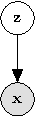
\includegraphics{media/directed_graphical_model}
  \caption{Directed graphical model}
  \label{fig:dgm}
  \medskip
  \small
  The latent variable $z$ is a stochastic dependency of the observed data $x$.
\end{figure}


\newpage
%Inverting $p(x|z)$ yields $p(z|x)$ which is one of the main tasks of some generative models, for example the VAE \ref{sec:vae}.


%After a short overview of different approaches and methods and an introductory example with the sigmoid belief net (SBN), we will take a closer look at two recent promising frameworks, the variational autoencoder (VAE \ref{sec:vae}) and the generative adversarial network (GAN \ref{sec:gan}).



%Generative models are one of the most promising ways to perform unsupervised learning (citation needed).
%More specifically, generative modelling assumes a hidden structure $z$ explaining the input data $x$.
%This assumption is reasonable given the following examples:\\




%Generative models have been proposed as one of the most promising approaches towards
%learning representations of real world data by some of the leading researchers (YannLeCun, OpenAI blogpost).

%In recent years supervised learning has yielded impressive results,
%however for these models to succeed huge amount of labelled data is needed.
%Unsupervised learning, that is learning from unlabelled data, has been expressed
%as one hurdles toward general articial intelligence (citation needed).
%Early approaches toward this problem however have shown that these problems are very hard to learn (intractable?).

%In generative models the approach is different in a way that
%we search for a good internal representation of the data.
%This resembles the way humans learn about the world where we incrementally build
%a model of the world.


